\section{Results}
\label{sec:results}

In this section we present the main results of this work, namely the determination
of the photon PDF $\gamma(x,Q^2)$ from a fit to the HERA structure functions
and ATLAS high-mass Drell-Yan cross-sections.

Using the NNLO fit settings discussed in Sect.~\ref{sec:fitsettings}, we find
a $\chi^{2}/N_{\rm dof} = 1.18$,
with a partial $\chi^2/N_{\rm dof} = 1.15$ for the high-mass Drell-yan data.
%
First of all we present our results for the photon PDF, and then the impact
of the DY measurements on the quark and gluon PDF.
%
In Fig.~\ref{photon_zoom} we show our results
for $\gamma(x,Q^2)$ for $Q^2=10^4$ GeV$^2$,
compared with LUXqed~\cite{Manohar:2016nzj}, HKR~\cite{Harland-Lang:2016apc}
and NNPDF3.0QED.
%
The comparison is restricted to the range $0.05 \le x \le 0.3$ corresponding
to the region where the fitted Drell-Yan measurements have direct kinematic sensitivity
to the photon PDF.
%
For NNPDF3.0QED, we show the 68\% CL uncertainty, while for LUXqed the uncertainty band
is obtained by adding in quadrature all the model variations.

%%%%%%%%%%%%%%%%%%%%%%%%%%%%%%%%%%%%%%%%%%%%%%%%%%%%%%%%
\begin{figure}[h]
\includegraphics[width=7cm]{figs/photon_comp_10000.pdf} 
\caption{Comparison between $\gamma(x,Q^2)$ at $Q^2=10^4$ GeV$^2$ in the present
  analysis with the corresponding results from NNPDF3.0QED, LUXqed and HKR.}
\label{photon_zoom}
\end{figure}
%%%%%%%%%%%%%%%%%%%%%%%%%%%%%%%%%%%%%%%%%%%%%%%%%%%%%%%%

From the results of Fig.~\ref{photon_zoom} we find that in the region where the HMDY data is
sensitive to the photon PDF, there is good agreement between the four determinations.
%
As compared to NNPDF3.0QED, the PDF uncertainties in the current analysis are reduced, though
they are still not competitive with those of LUXqed.
%
We also note the excellent agreement between the LUXqed and the HKN determinations.

We now turn the comparison to the quark and gluon PDFs.
%
Here we will compare a reference fit with the same settings as in Sect.~\ref{sec:fitsettings}
but with only the HERA inclusive structure function data with the results of this work,
which also include the ATLAS high-mass DY measurements.
%
We do not attempt to compare as well with the global fits, since our motivation here is only to
gauge the impact on quarks and gluons of the high-mass Drell-Yan data.

Fig.~\ref{PDF_7.5GeV}
shows the PDF distributions $x_{u_v},xd_{d_v},x\bar{u}, x\bar{d}, xg$ at $Q^{2}$ = 7.5$^{2}$ GeV$^{2}$,
with the MC experimental uncertainties

After this comparison at the level of PDFs, we move to a comparison between the theoretical
predictions and the high-mass Drell-Yan measurements.
%
In Fig.~\ref{hmDY_2D} we show the
comparison between the ATLAS high-mass Drell Yan data and the NNLO fit predictions
for the first bin of the $(y_{ll},m_{ll})$ distribution.
%
In the lower panel we shows the ratio of theory over data, where the yellow band
  corresponds to the correlated systematic uncertainties.

%%%%%%%%%%%%%%%%%%%%%%%%%%%%%%
\begin{figure}[h]
\centering
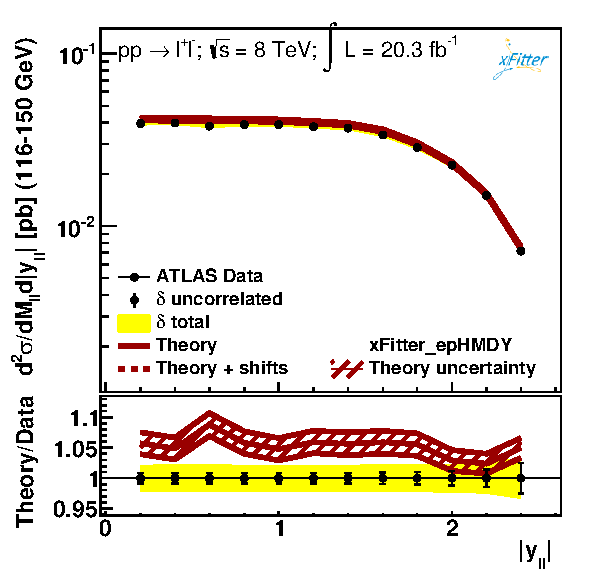
\includegraphics[width=7cm]{figs/data_1.pdf} 
\caption{Comparison between the ATLAS high-mass Drell Yan data and the NNLO fit predictions
  for the first bin of the $(y_{ll},m_{ll})$ distribution.
  %
  The lower panel shows the ratio of theory over data, where the yellow band
  corresponds to the correlated systematic uncertainties.
  %
  The band around the theory prediction corresponds to the total
  theory uncertainty from the PDF fit.
}
\label{hmDY_2D}
\end{figure}
%%%%%%%%%%%%%%%%%%%%%%%%%%%%%%%

The values of the $\chi^2$ for the HERA data and for
the high-mass DY data for the NNLO fit
are summarized in Table~\ref{tab:chi2fit}.
%
As can be seen, the agreement between data and the NNLO theory
is very good for all the $m_{ll}$ of the 8 TeV Drell-Yan data.
%
For the sum of all the five rapidity bins, we find a $\chi^2=55$
for 48 data points.
%
The quality of the agreement with the HERA inclusive structure functions
is similarly good.

%%%%%%%%%%%%%%%%%%%%%%%%%%%%%%%%%%%%%%%%%%%%
\begin{table}[h]
  \centering
  \begin{tabular}{|c|c|}
    \hline
    Dataset  &   $\chi^2$ \\
    \hline
    \hline
    hmDY  116 GeV $\ge y\ge $ 150 GeV  &  9.3/12 \\
    hmDY  150 GeV $\ge y\ge $ 200 GeV  &  17/12 \\
    hmDY  200 GeV $\ge y\ge $ 300 GeV  &  17/12 \\
    hmDY  300 GeV $\ge y\ge $ 500 GeV  &  3.8/6 \\
    hmDY  500 GeV $\ge y\ge $ 1500 GeV  &  4.2/6 \\
    \hline
    Correlated $\chi^2$ & 4.98 \\
    Log penalty $\chi^2$  & -0.0004 \\
    \hline
    \hline
    Total  & 55/48 \\
    \hline
    \end{tabular}
  \caption{$\chi^{2}$ for high-mass Drell Yan data for the NNLO fit.
    %
    We show the results for the individual $m_{ll}$ bins
    are well as for the total dataset.
\label{tab:chi2fit}
  }
\end{table}
%%%%%%%%%%%%%%%%%%%%%%%%%%%%%%%%%%%


Check the effect of the various variations on the photon PDF, but separately variation per variation,
showing the most important ones, and not stacking the error into a common error band


An important cross-check of the robustness of the estimated uncertainty for the photon
PDF in this analysis is provided by the comparison of the Monte Carlo method
with the Hessian method.
%
In Fig.~\ref{fig:photon_mc_vs_hessian} we show this comparison,
which indicates a reasonable agreement between the two methods.
%
In particular, the central values of the photon obtained with the two fitting
techniques are quite similar to each other.

%%%%%%%%%%%%%%%%%%%%%%%%%%%%%%
\begin{figure}[h]
\centering
\includegraphics[width=7cm]{figs/photon_mc_vs_hessian} 
\caption{Comparison between $x\gamma(x,Q^2)$ obtained with the
  Monte Carlo method with that from the Hessian method,
  at $Q^2=10^4$ GeV$^2$.
  %
  In both cases the PDF error band corresponds to the 68\% confidence level
  uncertainties. {\bf remove all other bands, update labels.}
}
\label{fig:photon_mc_vs_hessian}
\end{figure}
%%%%%%%%%%%%%%%%%%%%%%%%%%%%%%%

Another interesting question that our analysis allows addressing is what is
the impact of the high-mass Drell-Yan 8 TeV measurements on the quark and gluon
PDFs.
%
For this purpose, 
